\documentclass[border=10pt]{standalone}

\usepackage{tikz}
\usepackage{tikzsymbols}
\usetikzlibrary{calc,patterns,shapes.geometric}

\def\centerarc[#1](#2)(#3:#4:#5){\draw[#1] ($(#2)+({#5*cos(#3)},{#5*sin(#3)})$) arc (#3:#4:#5);}

\begin{document}
	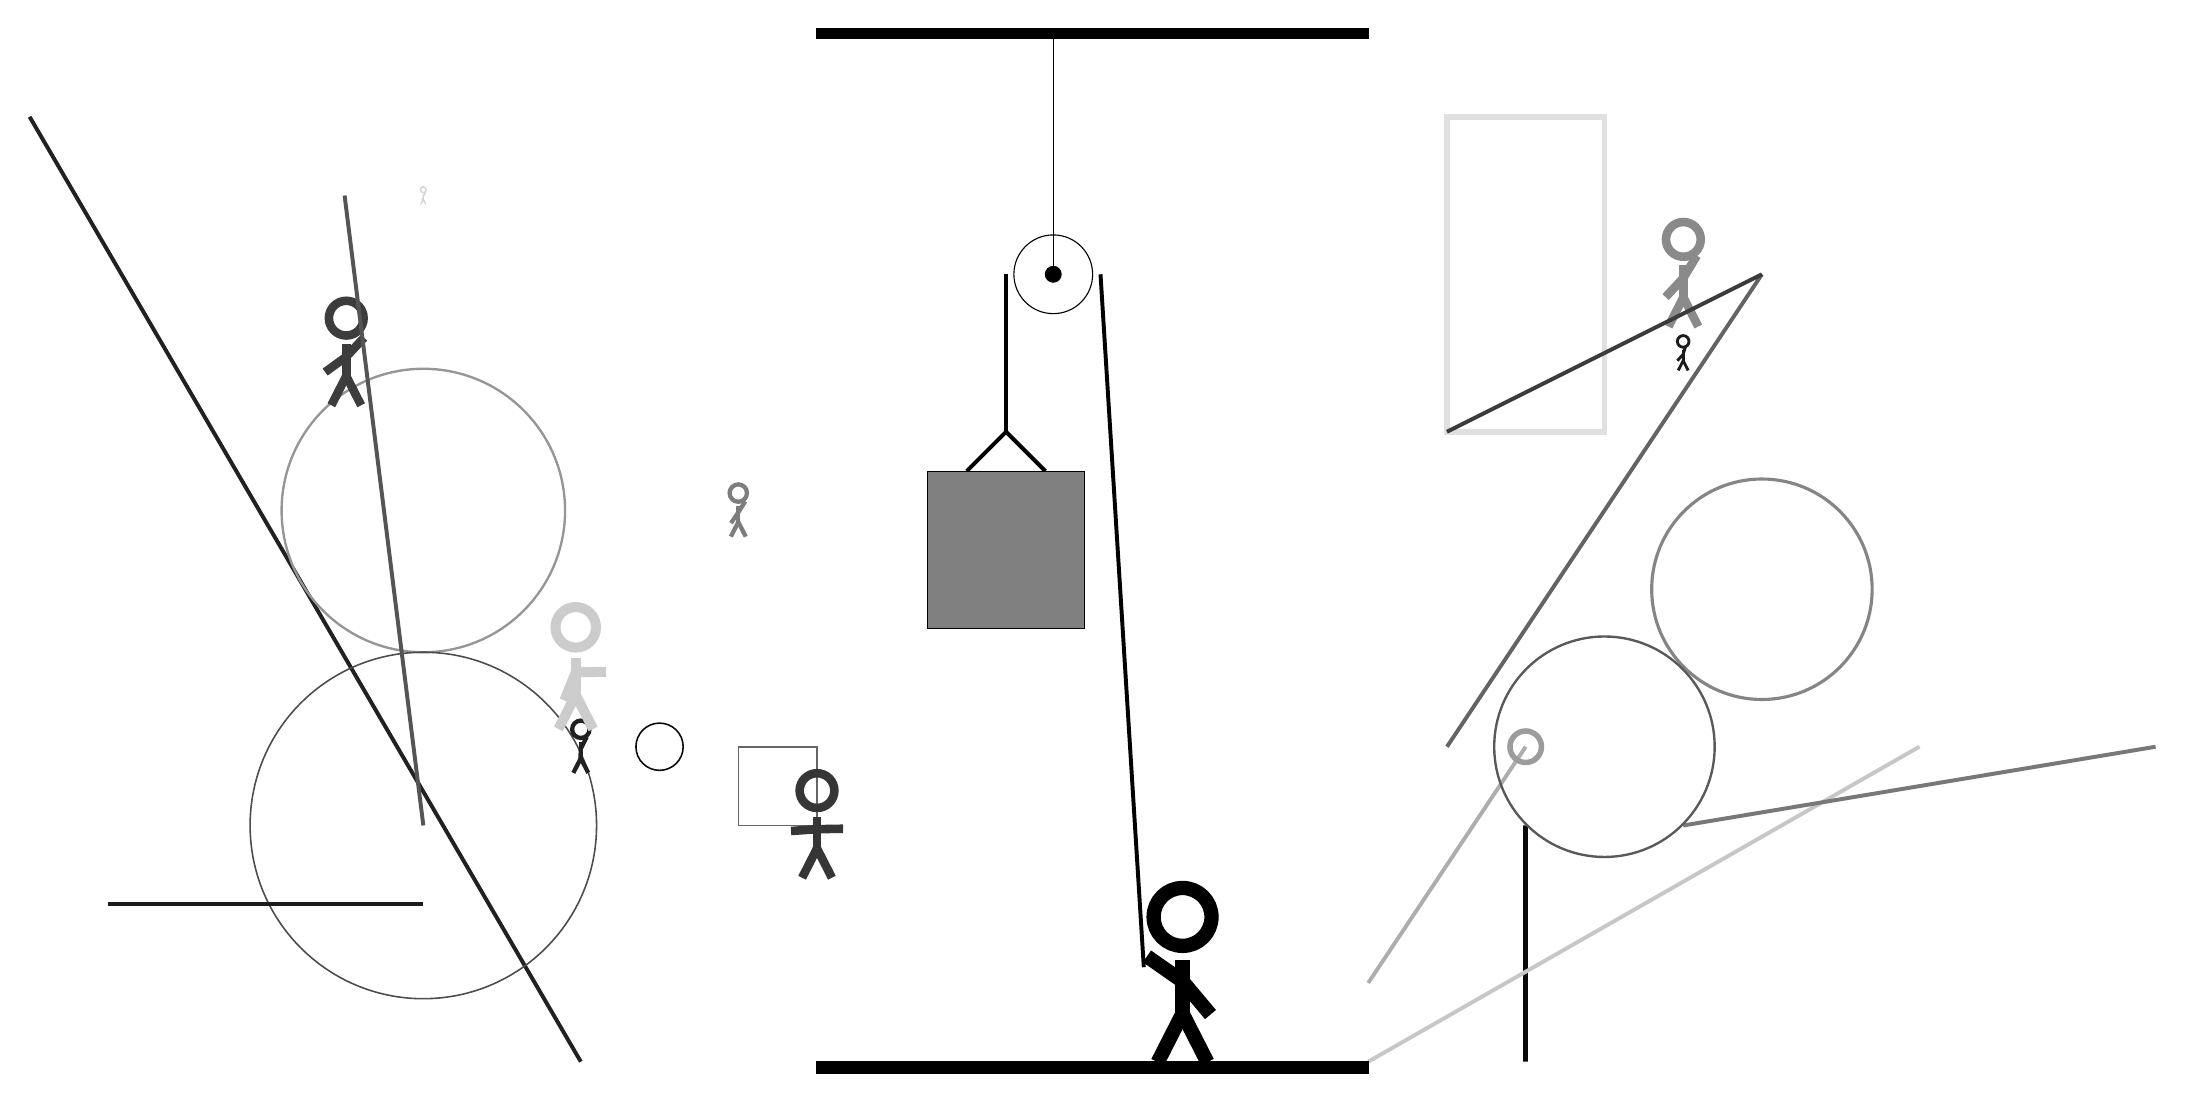
\begin{tikzpicture}
		%%%%% START %%%%%
		
		\draw[fill=black] (-2, 10) rectangle (5, 10.125);
		
		\draw[line width=0.7mm, color=black!12] (6, 9) rectangle (8, 5);
		
		\draw[line width=0.5mm, color=black!32](5, -2) -- (7, 1);
		\draw[line width=0.6mm, color=black!96] (7, 0) rectangle (7, -3);
		\draw[line width=0.5mm, color=black!87](-5, -3) -- (-12, 9);
		
		\node[line width=0.5mm, color=black!51] at (-3, 4) {\Strichmaxerl[3][56][58]};
		\draw [line width=0.2mm, color=black!96](-4, 1) circle (0.3);
		\draw[line width=0.5mm, color=black!61](6, 1) -- (10, 7);
		\draw [line width=0.3mm, color=black!41](-7, 4) circle (1.8);
		\draw[line width=0.2mm, color=black!60] (-3, 0) rectangle (-2, 1);
		\draw [line width=0.2mm, color=black!70](-7, 0) circle (2.2);
		\node[line width=0.7mm, color=black!89] at (9, 6) {\Strichmaxerl[2][48][73]};
		\node[line width=0.3mm, color=black!46] at (9, 7) {\Strichmaxerl[6][47][59]};
		\node[line width=0.6mm, color=black!79] at (-2, 0) {\Strichmaxerl[6][4][1]};
		
		\node[line width=0.3mm, color=black!87] at (-5, 1) {\Strichmaxerl[3][88][63]};
		\draw[line width=0.5mm, color=black!22](5, -3) -- (12, 1);
		\node[line width=0.4mm, color=black!20] at (-5, 2) {\Strichmaxerl[7][68][1]};
		\draw[line width=0.5mm, color=black!53](9, 0) -- (15, 1);
		
		\draw [line width=0.7mm, color=black!39](7, 1) circle (0.2);
		\node[line width=0.4mm, color=black!76] at (-8, 6) {\Strichmaxerl[6][36][47]};
		\draw [line width=0.4mm, color=black!48](10, 3) circle (1.4);
		\draw[line width=0.5mm, color=black!77](10, 7) -- (6, 5);
		
		\node[line width=0.5mm, color=black!17] at (-7, 8) {\Strichmaxerl[1][73][61]};
		\draw[line width=0.5mm, color=black!89](-7, -1) -- (-11, -1);
		\draw[line width=0.5mm, color=black!67](-7, 0) -- (-8, 8);
		\draw [line width=0.3mm, color=black!65](8, 1) circle (1.4);
		
		
		\draw (1, 7) circle (0.5);
		\draw[fill=black] (1, 7) circle (0.1);
		\draw (1, 10) -- (1, 7);
		
		\draw[line width=0.5mm] (-0.1, 4.5) -- (0.4, 5.0) -- (0.9, 4.5);
		\draw[fill=black!50] (-0.6, 4.5) rectangle (1.4, 2.5);
		
		\draw[line width=0.5mm] (0.4, 7) -- (0.4, 5.0);
		\centerarc[line width=0.5mm](1, 7)(0:180:0.6);
		\draw[line width=0.5mm](1.6, 7) -- (2.15, -1.8);
		
		\node at (2.6, -1.9) {\Strichmaxerl[10][-35][-50]};
		
		\draw[fill=black] (-2, -3) rectangle (5, -3.15);
		
		%%%%% END %%%%%
	\end{tikzpicture}
\end{document}